\subsection{Neuron models}

Mathematical models for the membrane potential behaviour started appearing in the early 1900. They range from the extremely detailed ones that consist of several differential equations to simple ones with just one or two, and they all model the electrical properties of the nerve cells. 

A particular group of models (self-compartment) describes the neuron as an isopotential sphere, that is, all its surface has the same electrical potential (Figure~\ref{fig:neuro:isopotential})~\cite{dayan2001theoretical}.

\begin{figure}[hbt]
  \begin{center}
    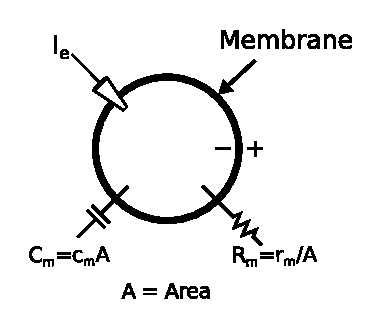
\includegraphics[width=0.45\textwidth]{iso_electrical_model}
    \caption{Diagram of the isopotential neuron. Adapted from \emph{Theoretical Neuroscience} by Dayan and Abbott~\cite{dayan2001theoretical}.}
    \label{fig:neuro:isopotential}
  \end{center}
\end{figure}

Since the neuron is modelled as a sphere, the membrane \emph{capacitance} $C_{m}$ and \emph{resistance} $R_{m}$ are specified in relation to its area $A$.

\begin{align}
R_{m} = r_{m}/A \\
C_{m} = c_{m}A
\end{align}
where $r_{m}$ and $c_{m}$ are the resistance and capacitance per unit area, 
respectively. Their values are $r_{m} \approx 1M \Omega mm^{2}$ and $c_{m} 
\approx 10nF/mm^{2}$. The basic relations of the electrical properties of the membrane are shown in  
Fig.~\ref{fig:neuro:isopotential}, are as follows:

\begin{align}
\Delta V &= I_{e}R_{m} \label{eq:neuro:volt-shift}\\[0.5em]
Q &= C_{m}V \label{eq:neuro:charge} \\[0.5em]
C_{m}\frac{dV}{dt} &= \frac{dQ}{dt} \label{eq:neuro:cap-curr}
\end{align}

When the membrane's potential changes, it does so according to Eq.~\ref{eq:neuro:volt-shift}. Variable $Q$ is the membrane's electrical charge which is proportional to the product of its voltage and capacitance, as seen in Eq.~\ref{eq:neuro:charge}.
Currents originated by ion channels are thought to be linear, and can be modelled using Ohm's law
\begin{equation}
i_{x} = g_{x}(V - E_{x}) 
\label{eq:neuro:single-channel-curr}
\end{equation}
where $E_{x}$ is the \emph{reverse potential} due to ion exchange in channel $x$ and $g_{x}$ is the per unit area conductance of the channel. The total membrane current due to channels (per unit area) will be 
\begin{equation}
i_{m} = \sum_{x} i_{x} = \sum_{x} g_{x}(V - E_{x}) \label{eq:neuro:total-channel-curr}
\end{equation}

For the total membrane current due to ion channels, Eq. \ref{eq:neuro:total-channel-curr} has to be multiplied by total area $A$.
The right hand side of Eq.~\ref{eq:neuro:cap-curr} is the total current in the membrane. Since we are adding an external current $I_{e}$ and is of opposite direction to $I_{m}$, the total current in the membrane is
\begin{equation}
I_{T} = I_{e} - I_{m} 
\label{eq:neuro:total-curr}
\end{equation}

Combining equations~\ref{eq:neuro:cap-curr}~and~\ref{eq:neuro:total-curr} with the fact that $i=dQ/dt$, gives the basic equation used by most self-compartment models~\cite{dayan2001theoretical}.
\begin{align}
C_{m} \frac{dV}{dt} &= I_{e} - I_{m} 
\label{eq:neuro:basic-self-compartment} \\[0.5em]
c_{m} \frac{dV}{dt} &= \frac{I_{e}}{A} - i_{m}
\label{eq:neuro:basic-pu-self-compartment}
\end{align}


\subsubsection{Leaky Integrate-and-fire}
This is one of the oldest neuron models, but it's still being used due to its simplicity. In the passive \emph{integrate-and-fire} all the membrane conductances are modelled by a single term $G_{L}$ (Equation~\ref{eq:neuro:passive-int-n-fire}).
\begin{equation}
C_{m}\frac{dV}{dt} = I_{e} - G_{L}\left( V - E_{L} \right) 
\label{eq:neuro:passive-int-n-fire}
\end{equation}
the rightmost term is also known as \emph{leak current}. If Eq.~\ref{eq:neuro:passive-int-n-fire} is multiplied by the membrane resistance $R_{m}$, we obtain
\begin{equation}
\tau_{m}\frac{dV}{dt} = R_{m}I_{e} - V + E_{L}  
\label{eq:neuro:passive-R-int-n-fire}
\end{equation}
Integrating Eq. \ref{eq:neuro:passive-R-int-n-fire} results in an expression for the voltage behaviour under non-spiking conditions.
\begin{equation}
V\left( t \right) = E_{L} + R_{m}I_{e} + 
                    \left( V\left( 0 \right) - E_{L} - R_{m}I_{e}\right) e^{ -t/\tau_{m}}
\label{eq:neuro:passive-V-int-n-fire}
\end{equation}
Spiking behaviour is added artificially once $V(t)$ reaches a certain threshold, afterwards it's reset back to $V(0)$.


\subsubsection{Hodgkin-Huxley}
In 1952, Hodgkin and Huxley published a paper that reflected their ground-breaking experimental work on the axon of the squid~\cite{hodgkin-huxley}. They found that the currents in the membrane are mainly due to changes in the concentration of three ions: potassium ($K^{+}$), sodium ($Na^{+}$) and chlorine ($Cl^{-}$). The first two are related to voltage dependant conductance and the last to a leak current. Under these considerations, Eq. \ref{eq:neuro:basic-self-compartment} becomes~\cite{dynamical-systems-Izhikevich2007}:
\begin{equation}
C_{m}\frac{dV}{dt} = I_{e} - g_{K}  n^{4} (V - E_{K}) 
                           - g_{Na} m^{3}h(V - E_{Na})
                           - g_{L}        (V - E_{L})
\label{eq:neuro:hodgkin-huxley}
\end{equation}
the variables $n$, $m$ and $h$ have the following behaviour
\begin{align}
\frac{dn}{dt} &= \alpha_{n}(V) (1 - n) - \beta_{n}(V) n \\[0.5em]
\frac{dn}{dt} &= \alpha_{m}(V) (1 - m) - \beta_{m}(V) m\\[0.5em]
\frac{dn}{dt} &= \alpha_{h}(V) (1 - h) - \beta_{h}(V) h
\end{align}
%and
%\begin{align}
%\alpha_{n}(V) &= 0.01\frac{10 - V}{e^{(10 - V)/10} - 1 } \qquad \qquad 
%\beta_{n}(V) = 0.125 e^{-V/80} \\[0.5em]
%%
%\alpha_{m}(V) &= 0.1\frac{25 - V}{e^{(25 - V)/10} - 1 } \qquad \qquad 
%\beta_{m}(V) = 4 e^{-V/18} \\[0.5em]
%%
%\alpha_{h}(V) &= 0.07\frac{10 - V}{e^{(10 - V)/10} - 1 } \qquad \qquad 
%\beta_{h}(V) = 0.125 e^{-V/80}
%\end{align}

The Hodgkin-Huxley model is one of the most detailed so far, it has served as inspiration and foundation of many studies. The main issue with this level of detail is that it comes at a price, it's computationally expensive; so, for systems simulating a big number of neurons the hardware has to be equally powerful.

\subsubsection{Simple model}
The dynamics of the Hodgkin-Huxley were studied using bifurcation diagrams and approximated by \citeauthor{fitzhugh1961impulses}~\cite{fitzhugh1961impulses}. Using similar ideas and techniques, \citeauthor{izhikevich2003simple} developed what he named the \emph{simple model} of spiking neurons~\cite{izhikevich2003simple}. This model emulates the dynamics of membrane voltage on the sub-threshold area, for modelling the spike behaviour comes at the cost of tiny time steps that increase the computational cost. \citeauthor{izhikevich2003simple}'s simple model consists of a pair of equations:
\begin{align}
  \frac{dv}{dt} &= 0.04v^{2} + 5v + 140 - u - I \\[0.5em]
  \frac{du}{dt} &= a(bv - u)
\end{align}
where $v$ represents membrane voltage and $u$ a negative feedback to $v$. The rising part of spiking behaviour is produced by the equations, though an artificial voltage reset is needed afterwards. When variable $v$ reaches 30 $mV$ or more, variables $v$ and $u$ are set as follows
\begin{equation}
  v = c \qquad u = u + d
\end{equation}
Parameters $a$, $b$, $c$ and $d$ are dimensionless and time has a $ms$ resolution. Changes in  the values of the parameters result in different types of neuron responses~\cite{dynamical-systems-Izhikevich2007}. 

The simple model has, at least, two advantages: first, many observed neural behaviours can be replicated by modifying the model's parameters; and second, it keeps biological plausibility while having low computational cost~\cite{izhikevich2004model}. This model seems to be the right candidate for large-scale, biologically-plausible and energy-efficient systems.












